\documentclass[11pt,a4paper]{report}
\usepackage[utf8]{inputenc}
\usepackage[french]{babel}
\usepackage[T1]{fontenc}
\usepackage{amsmath}
\usepackage{amsfonts}
\usepackage{amssymb}
\usepackage{xcolor}

\usepackage{geometry}
\geometry{hmargin=2.5cm,vmargin=1.5cm}
\usepackage{wasysym}
\usepackage{graphicx}

\author{Mathieu Sarrat}
\title{LP10 - Induction électromagnétique}

\makeatletter
\renewcommand{\thesection}{\@arabic\c@section}
\makeatother


\begin{document}
\maketitle

\subsection{Pré-requis}
\begin{itemize}
	\item \'Equations de Maxwell en régime stationnaire
	\item Force de Lorentz et force de Laplace
	\item Champ magnétique généré par un solénoïde infini
\end{itemize}

\subsection{Objectifs}
\begin{itemize}
	\item Introduire la notion d'induction électromagnétique
\end{itemize}

\newpage
\section{Introduction}



\newpage
\section{Mise en évidence}

\subsection{Champ électromagnétique, force de Lorentz et relativité galiléenne}

Rappelons tout d'abord qu'une particule chargée $q$ plongée dans un champ électromagnétique $(\bold{E},\bold{B})$ est soumise à la force de Lorentz
\begin{equation}
	\bold{F} = q \left(\bold{E}+\bold{v}_\mathcal{R}\times\bold{B}\right),
\end{equation}
où $\bold{v}_\mathcal{R}$ désigne la vitesse de la particule \textbf{dans le référentiel d'étude}. Ainsi, par rapport à un autre référentiel $\mathcal{R}'$, la force de Lorentz s'écrit
\begin{equation}
	\bold{F}' = q' \left(\bold{E}'+\bold{v}_{\mathcal{R}'}\times\bold{B}'\right),
\end{equation}
où figure $\bold{v}_{\mathcal{R}'}$ la vitesse de la particule par rapport à $\mathcal{R}'$.

En relativité galiléenne, la charge électrique et la force sont des grandeurs invariantes par changement de référentiel galiléen. Si $\mathcal{R}$ et $\mathcal{R}'$ sont deux référentiels galiléens,
\begin{equation}
	q' = q \qquad \text{et} \qquad \bold{F}' = \bold{F}. 
\end{equation}

En utilisant la loi de composition des vitesses galiléenne $\bold{v}_{\mathcal{R}} = \bold{v}_{\mathcal{R}'} + \bold{V}_{\mathcal{R}'/\mathcal{R}}$, où $\bold{V}_{\mathcal{R}'/\mathcal{R}}$ désigne la vitesse d'entraînement, on trouve les formules de transformation suivantes,
\begin{equation}
	\bold{B}' = \bold{B} \qquad \text{et} \qquad \bold{E}' = \bold{E} + \bold{V}_{\mathcal{R}'/\mathcal{R}}\times\bold{B}.
\end{equation}

La partie électrique de l'interaction n'est pas perçue de la même manière par un observateur placé dans $\mathcal{R}'$ et un autre placé dans $\mathcal{R}$. Lorsque des charges se déplacent dans un conducteur en mouvement, elles ressentent un champ électrique dépendant directement du mouvement du conducteur dans le champ magnétique. Le champ électrique et le champ magnétique sont étroitement liés, d'où l'importance accordée au concept plus général de champ électromagnétique $(\bold{E},\bold{B})$. Ceci est encore plus vrai en relativité restreinte.

\subsection{L'expérience de Faraday (1831)}

Soient deux circuits électriques $C_1$ et $C_2$ placés de telle sorte que le flux du champ magnétique créé par l'un à travers l'autre soit suffisamment important (on introduit une bobine dans chacun de ces circuits pour pouvoir générer un champ magnétique significatif). Le circuit $C_1$ est alimenté par un générateur et comporte un interrupteur $K$. Le circuit $C_2$ ne comporte qu'un galvanomètre permettant de mesurer l'intensité du courant électrique mais aussi son sens. Les notations utilisées sur le schéma représentent le sens positif des courants $i_1$ et $i_2$. Nous allons effectuer plusieurs manipulations pour mettre en évidence le phénomène d'induction électromagnétique.\\

\subsubsection{Circuits fixes :}

Expérience 1 :
\begin{itemize}
	\item Initialement : interrupteur $K$ ouvert, donc $i_1 = 0$ et $i_2 = 0$
	\item Manip : fermeture de $K$ et augmentation progressive du courant $i_1$ débité par le générateur. Mesure de $i_1 > 0$ dans $C_1$ et mesure de $i_2 < 0$ tant que $i_1$ varie.
\end{itemize}

Expérience 2 : suite de 1
\begin{itemize}
	\item Initialement : interrupteur $K$ fermé, $i_1 > 0$ et constant mesuré, $i_2 = 0$
	\item Manip : diminuer $i_1$ et constater l'apparition de $i_2 > 0$ dans $C_2$
\end{itemize}
	
Expérience 3 : inverser la polarité du générateur et refaire l'expérience 1, constater l'inversion des signes des courants $i_1$ et $i_2$.

\subsubsection{Circuits mobiles :}

$C_2$ peut bouger par rapport à $C_1$.

Expérience 1 :
\begin{itemize}
	\item Initialement $K$ fermé, donc $i_1 > 0$ et $i_2 = 0$.
	\item On éloigne $C_1$ de $C_2$ : $i_2 > 0$ circule dans $C_2$ tant qu'il y a du mouvement. 
\end{itemize}

Expérience 2 :
\begin{itemize}
	\item Initialement $K$ fermé, donc $i_1 > 0$ et $i_2 = 0$.
	\item On éloigne $C_2$ de $C_1$ : $i_2 > 0$ circule dans $C_2$ tant qu'il y a du mouvement.
\end{itemize}
Le courant induit est d'autant plus intense que le déplacement est rapide.

\subsection{Définition de la force électromotrice induite}

\textcolor{red}{Consignes : aller directement à l'expression de $e(t)$ dans le cas général, en expliquant la signification de chaque grandeur ($+$ schéma), détailler le cas du circuit fixe et expliquer la relation entre les deux formules à la lumière de la transformation de Galilée de $(\bold{E},\bold{B})$. Expliquer que $e(t)$ est calculée à partir du travail électromoteur (le travail de la force de Lorentz servant à mettre en mouvement les charges dans le conducteur).}

\subsubsection{Travail fourni par le champ électromagnétique}

L'apparition d'un courant dans le conducteur est liée à la mise en mouvement des charges sous l'effet de la force de Lorentz. Considérons un élément de volume matériel $d\mathcal{V}$ centré au point $M$ appartenant au conducteur. Ce morceau de conducteur est animé d'une vitesse $\bold{V}$ dans le référentiel $\mathcal{R}$ et est plongé dans un champ électromagnétique $(\bold{E},\bold{B})$. Cet élément contient deux types de charges électriques :
\begin{itemize}
	\item des charges fixes (les ions du réseau), de densité volumique de charge $\rho_f$. Elles se déplacent ensemble, avec la vitesse $\bold{V}$ de l'élément $d\mathcal{V}$,
	\item des charges mobiles (les électrons de conduction), de densité volumique de charge $\rho_m$ et qui se déplacent à la vitesse $\bold{u}+\bold{V}$, où $\bold{u}$ désigne la vitesse de dérive des électrons dans le conducteur, responsable du courant électrique. C'est la vitesse moyenne des électrons dans le câble (leur vitesse exacte à laquelle on retire leur vitesse d'agitation thermique, aléatoire). La densité volumique de courant s'écrit donc $\bold{J} = \rho_m \bold{u}$.
\end{itemize}
On suppose que le conducteur est électriquement neutre : $\rho_m + \rho_f = 0$.\\


La force agissant sur l'ensemble des charges de $d\mathcal{V}$ s'écrit donc
\begin{equation}
	d\bold{F}_L = d\bold{F}_m + d\bold{F}_f = \rho_m d\mathcal{V} \left[\bold{E}+\left(\bold{u}+\bold{V}\right)\times\bold{B}\right]   
	+ \rho_f d\mathcal{V} \left[\bold{E}+\bold{V}\times\bold{B}\right].
\end{equation}
\textit{Remarque : la force totale $\bold{F}_L = \int_\mathcal{V} d\bold{F}_L$, rappelons-le, est appelée force de Laplace.}\\

Entre $t$ et $t+dt$ les charges contenues dans $d\mathcal{V}$ reçoivent de la force de Lorentz une énergie
\begin{align*}
	\delta^2 W & 
	= \rho_m d\mathcal{V}\left[\bold{E}+\left(\bold{u}+\bold{V}\right)\times\bold{B}\right]
	\cdot\left(\bold{u}+\bold{V}\right)dt 
	+\rho_f d\mathcal{V}\left[\bold{E}+\bold{V}\times\bold{B}\right]\cdot\bold{V}dt\\
	& = d\mathcal{V}dt\left[\rho_m \bold{E}\cdot\bold{u} 
	+ \underbrace{\left(\rho_m + \rho_f\right)}_{\displaystyle{= 0}}
	\bold{E}\cdot\bold{\bold{V}}\right] 
	= \rho_m \bold{E}\cdot\bold{u}\;d\mathcal{V}dt\\
	\delta^2 W & = \bold{E}\cdot\bold{J}\;d\mathcal{V}dt 
\end{align*}
Les autres termes sont nuls ou s'éliminent entre eux. On voit que la partie magnétique ne travaille pas : l'action de $\bold{B}$ sur les charges mobiles est entièrement transmise à l'ensemble des charges du conducteur sans pertes. L'ensemble du travail fourni aux charges l'est grâce au champ électrique.

Pour l'ensemble du conducteur, le travail reçu par les charges vaut
\begin{equation}
	\delta W = \int \delta^2 W = dt\iiint_\mathcal{V} \bold{E}\cdot\bold{J}\;d\mathcal{V}.
\end{equation}
Supposons un conducteur filiforme $C$ de section $S$ et donc par conséquent des champs homogènes sur toute la section du câble : $\bold{J}\;d\mathcal{V} = i\;d\bold{r}$
\begin{equation}
	\delta W = i\;dt \oint_C \bold{E}\cdot d\bold{r}
	\label{eq:travail_total}
\end{equation}

\subsubsection{Force électromotrice}

L'équation \eqref{eq:travail_total} permet de calculer le travail total fourni par le champ électromagnétique aux charges du matériau conducteur. Dans le cas générale, seule une partie de cette énergie sert à mettre les charges en mouvement dans le circuit : on parle de \textbf{travail électromoteur} $\delta W_m$. On définit la force électromotrice à partir 
de ce travail électromoteur :
\begin{equation}
	e(t) \equiv \frac{\delta W_m}{\delta q}.
\end{equation}

On calcule le travail électromoteur de la façon suivante. Pour un élément de conducteur $d\mathcal{V}$, ce travail se résume à
\begin{align}
	\delta^2_m W & = d\bold{F}_m \cdot \bold{u}\;dt\\
			   & = \rho_m d\mathcal{V} dt \left[\bold{E}+\left(\bold{u}+\bold{V}\right)\times\bold{B} \right]\cdot \bold{u}\\
			   & = d\mathcal{V} dt \left[\bold{E}+ \bold{V}\times\bold{B}\right]\cdot \bold{J}
\end{align}
puisque les charges dites fixes n'ont aucun mouvement dans $\mathcal{R}'$. Sur tout le circuit 
\begin{equation}
	\delta W_m  = dt \iiint_\mathcal{V} \left[\bold{E} + \bold{V}\times\bold{B}\right] \;d\mathcal{V}
			    = i\;dt \oint_C \left[\bold{E} +  \bold{V}\times\bold{B}\right]\cdot\;d\bold{r}
\end{equation}
la dernière équation étant vraie pour un conducteur filiforme $C$.\\

Par conséquent, dans un circuit en mouvement quelconque, déformable ou non, la force électromotrice a pour expression
\begin{equation}
	e(t) = \oint_C\left[\bold{E}(\bold{r}) + \bold{V}(\bold{r})\times\bold{B}(\bold{r})\right]\cdot d\bold{r}.
\end{equation}
où $\bold{V}(\bold{r})$ désigne la vitesse de l'élément de circuit situé au point $\bold{r}$.\\

Dans le cas où le circuit est immobile, cas particulier mais très important en termes d'applications pratiques, cette expression se réduit à
\begin{equation}
	e(t) = \oint_C \bold{E}(\bold{r})\cdot d\bold{r},
\end{equation}
c'est à dire à la circulation du champ électrique le long du circuit. En régime variable et contrairement à ce que l'on rencontre en électrostatique, cette circulation n'est pas nulle (nous le verrons plus loin).\\

\textbf{Remarque :} l'expression de $e(t)$ paraît dépendre du référentiel dans lequel on se place, puisque la vitesse du circuit intervient explicitement dans le calcul. En réalité, $e(t)$ (et c'est vérifié expérimentalement) est la même dans tout référentiel galiléen, du fait de l'invariance des lois physiques entre deux référentiels galiléens. \'A un instant donné et en un point $M$ quelconque du circuit, il est possible de définir un référentiel galiléen $\mathcal{R'}$ en translation dans $\mathcal{R}$. On peut alors utiliser les notations suivantes
\begin{equation}
	\bold{u} = \bold{u}_{/\mathcal{R}'} \qquad\text{et}\qquad \bold{V} \equiv \bold{V}_{\mathcal{R}'/\mathcal{R}}.
\end{equation}
On reconnaît alors sous l'intégrale l'expression du champ électrique $\bold{E}'$ perçu par une charge située au point $\bold{r}$ dans le conducteur, écrite en fonction des champs $\bold{E}$ et $\bold{B}$ relatifs au référentiel $\mathcal{R}$. Dans le référentiel où le circuit (s'il est indéformable) est immobile,
\begin{equation}
	e(t) = \oint_C \bold{E}'(\bold{r})\cdot d\bold{r} = \oint_C\left[\bold{E}(\bold{r}) + \bold{V}(\bold{r})\times\bold{B}(\bold{r})\right]\cdot d\bold{r}.
\end{equation} 

\textbf{Remarque :} on vérifie bien que la différence entre $\delta W$ et $\delta W_m$ correspond au travail des forces de Laplace :
\begin{equation}
	\delta^2 W - \delta^2 W_m = \rho_m \bold{E}\cdot\bold{u}\;d\mathcal{V}dt - \rho_m 					\left[\bold{E}+\bold{V}\times\bold{B}\right]\cdot\bold{u}\;d\mathcal{V}dt
\end{equation}
\begin{equation}
	\delta^2 W - \delta^2 W_m = - \rho_m \left[\bold{V}\times\bold{B}\right]\cdot\bold{u}\;d\mathcal{V}dt
\end{equation}
\begin{equation}
	\delta^2 W - \delta^2 W_m = \left[\bold{B}\times\bold{V}\right]\cdot\bold{J}\;d\mathcal{V}dt
\end{equation}
\begin{equation}
	\delta^2 W - \delta^2 W_m = \left[\bold{J}\times\bold{B}\right]\cdot\bold{V}\;d\mathcal{V}dt
\end{equation}
d'où 
\begin{equation}
	\delta W_L = \delta^2 W - \delta^2 W_m = dt\iiint \left[\bold{J}\times\bold{B}\right]\cdot\bold{V}\;d\mathcal{V}.
\end{equation}
Ces forces ne travaillent qu'en cas de mouvement d'une portion du circuit ou du circuit dans sa totalité.	

\newpage
\section{Lois de l'induction}

\subsection{Relations de Maxwell-Faraday et de Maxwell-Thomson}

\subsubsection{Relation de Maxwell-Faraday}
Une équation fondamentale de l'électromagnétisme permet de modéliser et de décrire le phénomène d'induction. Il s'agît de l'équation de Maxwell-Faraday (une des quatre équations de Maxwell), que nous écrirons sous sa forme locale (valable en tout point) :
	\begin{equation}
		\textbf{rot}\;\bold{E} + \frac{\partial\bold{B}}{\partial t} = 0.		
	\end{equation}

Cette équation est souvent qualifiée de \textbf{relation structurelle} du champ électromagnétique : les densités de charge et de courant n'interviennent pas dans son écriture. Cette équation permet de relier la création d'un champ électrique à la variation temporelle d'un champ magnétique, phénomène que nous avons mis en évidence dans la section précédente puisque nous avons relié l'apparition d'une force électromotrice à la variation du flux du champ magnétique.\\

Pour préciser les choses, établissons la formulation globale de cette loi : soit un contour quelconque $\mathcal{C}$ (qui peut ou non coïncider avec un circuit électrique $C$) sur lequel s'appuie une surface ouverte notée $\mathcal{S}$. L'intégration sur $\mathcal{S}$ de l'équation de Maxwell-Faraday conduit à
\begin{align}
   0 & =  \iint_\mathcal{S} \left[\textbf{rot}\;\bold{E} + \frac{\partial\bold{B}}{\partial t}\right]\cdot d\mathcal{S}\\
   	 & =  \oint_\mathcal{C} \bold{E} \cdot \;d\bold{r} + \iint_\mathcal{S}\frac{\partial\bold{B}}{\partial t}\cdot d\mathcal{S}
\end{align}
en appliquant le théorème de Stokes, $d\bold{r}$ désignant un élément de longueur du contour $\mathcal{C}$. On obtient finalement
\begin{equation}
	\oint_\mathcal{C} \bold{E} \cdot \;d\bold{r} = - \iint_\mathcal{S}\frac{\partial\bold{B}}{\partial t}\cdot d\mathcal{S}.
\end{equation}
	
En régime variable, le champ électrique n'est pas à circulation conservative, contrairement au régime stationnaire. La valeur de cette circulation dépend directement de la variation du champ magnétique au cours du temps. Les conséquences de cette équation sur la nature des potentiels électrique $V$ et magnétique $\bold{A}$ seront détaillées dans une leçon ultérieure.
	
\subsubsection{Relation de Maxwell-Thomson}
Il existe une seconde relation structurelle du champ électromagnétique, qui nous aidera à établir les lois de l'induction mais qui ne décrit pas ces phénomènes contrairement à Maxwell-Faraday. C'est la relation de Maxwell-Thomson, qui s'écrit, sous sa forme locale	
	\begin{equation}
		\text{div}\;\bold{B} = 0.
	\end{equation}
	
Soit un volume $\mathcal{V}$ quelconque (contenant ou non de la matière), délimité par une surface \textbf{fermée} $\mathcal{S}$. L'intégration sur $\mathcal{S}$ conduit à la formulation globale de la relation de Maxwell-Thomson :
	\begin{align}
   		0 & = \iiint \text{div}\;\bold{B} d\mathcal{V}\\
   	 	  & = \oiint \bold{B}\cdot d\bold{S} = \Phi. 
	\end{align}
	par application du théorème de Green-Ostrogradsky. Le flux total de champ magnétique $\Phi$ transitant à travers toute surface fermée $\mathcal{S}$ est nul : 
	l'équation de Maxwell-Thomson implique donc la \textbf{conservation du flux magnétique}. Si on divise $\mathcal{S}$ en deux parties $\mathcal{S}_1$ et $\mathcal{S}_2$, 
	cette relation implique que le flux sortant par $S_1$ revient par $S_2$ et vice-versa. C'est cette équation qui interdit l'existence d'un monopole magnétique en 
	électromagnétisme classique.
		
\subsection{Lois de l'induction}	
	
	\subsubsection{Expression générale de la force électromotrice induite}
	
	Reprenons notre circuit électrique $C$, qui peut être en mouvement dans le référentiel d'étude $\mathcal{R}$. On combine l'expression générale de la force électromotrice induite $e(t)$ avec la forme globale de l'équation de Maxwell-Faraday, appliquée à un contour $\mathcal{C}$ coïncidant avec le circuit $C$. Tout élément de contour $d\bold{r}$ coïncide avec un élément $d\bold{l}$ du circuit $C$ :
	
	\begin{align}
   		e(t)& =  \oint_\mathcal{C}\left(\bold{E} + \bold{V}\times\bold{B}\right)\cdot d\bold{l}   \\
   		    & =  \oint_\mathcal{C}\bold{E}\cdot d\bold{l} + \oint_\mathcal{C}\left(\bold{V}\times\bold{B}\right)\cdot d\bold{l} \\
   	 		& =  - \iint_\mathcal{S}\frac{\partial\bold{B}}{\partial t}\cdot d\mathcal{S} + \oint_\mathcal{C}\left(\bold{V}\times\bold{B}\right)\cdot d\bold{l}
	\end{align}
		
	On en déduit une expression générale de la force électromotrice induite $e(t)$ en fonction de la variation temporelle de $\bold{B}$. Cette expression ne fait appel qu'à des grandeurs, des contours et des surfaces bien définis à chaque instant dans le référentiel d'étude $\mathcal{R}$. La vitesse $\bold{V}$ désigne la vitesse d'un point du circuit $C$ (par rapport à $\mathcal{R}$) qui coïncide à l'instant $t$ avec un point du contour $\mathcal{C}$. Cette expression est valable quelque soit le mouvement du conducteur et dépend naturellement du référentiel choisi.\\
	
	On distingue deux contributions à la force électromotrice induite :
	\begin{itemize}
		\item une contribution liée à la seule variation temporelle de $\bold{B}$ (première situation présentée dans la première partie de la leçon). En effet, si le circuit est immobile, 
		$\bold{V} = 0$ en tout point de $C$ et par conséquent
		\begin{equation}
			e(t) = - - \iint_\mathcal{S}\frac{\partial\bold{B}}{\partial t}\cdot d\mathcal{S} = - \frac{d}{dt}\iint_\mathcal{S}\bold{B}\cdot d\mathcal{S} = - \frac{d\Phi}{dt}.
		\end{equation}
		En effet, si le circuit ne bouge pas il est forcément indéformable : la surface d'intégration est invariante au cours du temps.
		Cette situation est appelée \textbf{induction statique} (circuit fixe) ou \textbf{induction de Neumann}.
		
		\item une contribution liée au déplacement du conducteur. Ce déplacement peut être un déplacement d'ensemble ou une déformation du circuit. Si le champ magnétique est stationnaire,
			\begin{equation}
				\frac{\partial \bold{B}}{\partial t} = 0 \qquad \text{et donc} \qquad e(t) = \oint_\mathcal{C}\left(\bold{V}\times\bold{B}\right)\cdot d\bold{l}.
			\end{equation}
		On parle dans ce cas d'\textbf{induction motionnelle} ou encore d'\textbf{induction de Lorentz}. Une illustration classique de ce type d'induction est le problème des Rails de 				Laplace, que l'on traitera en détail en TD. Donnons cependant une brève présentation de ce système : un barreau conducteur est posé sur deux rails, également conducteurs. Le contact 			entre barreau et rails est glissant : le barreau se déplace le long des rails avec une vitesse $\bold{V} = V \bold{e}_x$. Le circuit est fermé par un voltmètre connecté entre les 				rails. On place le système dans un champ magnétique uniforme et stationnaire, de direction perpendiculaire au plan formé par les rails. Tant que le barreau bouge, le voltmètre mesure 		une force électromotrice que l'on peut calculer à partir de l'expression générale de $e(t)$. 
		\begin{figure}[h!]
		\begin{center}
			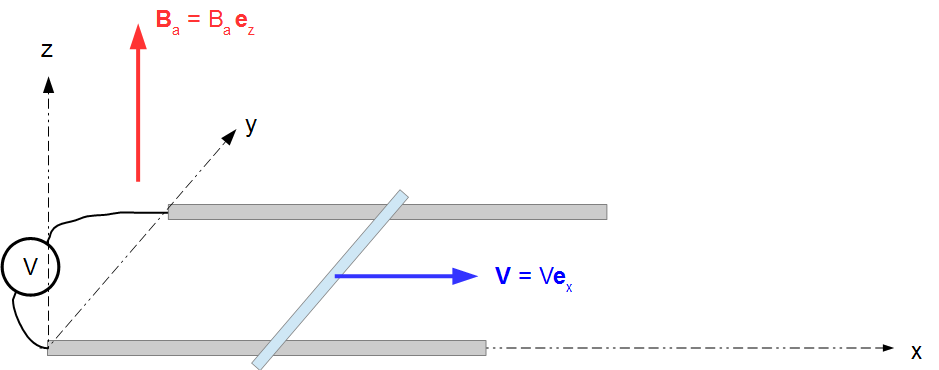
\includegraphics[scale = 0.4]{rails_Laplace.png}
			\caption{Rails de Laplace} 
			\label{fig:rails_Laplace}
		\end{center}
		\end{figure}
	\end{itemize}
	
	\subsubsection{Loi de Faraday et loi de Lenz}
	
	On ne s'intéresse ici qu'à des circuits électriques de constitution invariante dans le temps (pas de déformation du circuit au cours du temps, mais celui-ci peut se déplacer en bloc dans le référentiel d'étude $\mathcal{R}$). On a établi expérimentalement un lien entre la force électromotrice induite $e(t$) et la variation temporelle du flux magnétique $\Phi$ à travers le circuit. Essayons d'établir mathématiquement une relation entre ces deux grandeurs.\\
	
	Dans ce but, considérons un circuit $C$ auquel on superpose à chaque instant un contour $\mathcal{C}$ de sorte que le contour bouge avec le circuit avec la vitesse $\bold{V}$ par rapport au référentiel d'étude $\mathcal{R}$. Le champ magnétique $\mathcal{B}$ dans lequel est plongé le circuit dépend du temps et de la position (non stationnaire et non homogène).\\

	Mathématiquement :
	\begin{align}
		\frac{d\Phi}{dt} & = \frac{d}{dt}\iint_{\mathcal{S}(t)}\bold{B}(\bold{r},t)\cdot d\bold{\mathcal{S}}
					     & = \frac{\Phi(t+dt) - \Phi(t)}{dt}
					     & = \frac{1}{dt}\left[\iint_{\mathcal{S}(t+dt)}\bold{B}(\bold{r},t+dt)\cdot d\bold{\mathcal{S}} 
					     - \iint_{\mathcal{S}(t)}\bold{B}(\bold{r},t)\cdot d\bold{\mathcal{S}}\right]
	\end{align}

	On ajoute deux intégrales opposées pour faire apparaître deux variations de flux, 
	\begin{equation}
		\frac{d\Phi}{dt} = \frac{1}{dt}\iint_{\mathcal{S}(t+dt)}\left[\bold{B}(\bold{r},t+dt)-\bold{B}(\bold{r},t)\right]\cdot d\bold{\mathcal{S}} 
						 + \frac{1}{dt}\left[\iint_{\mathcal{S}(t+dt)}\bold{B}(\bold{r},t)\cdot d\bold{\mathcal{S}}
						 -\iint_{\mathcal{S}(t)}\bold{B}(\bold{r},t)\cdot d\bold{\mathcal{S}} \right]
	\end{equation}
	\begin{itemize}
		\item la première due à la variation temporelle intrinsèque de $\bold{B}$,
		\item la seconde due au déplacement de $C$ à travers la structure de $\bold{B}$.
	\end{itemize}

	On peut démontrer que, puisque $\text{div}\;\bold{B} = 0$,
	\begin{equation}
		\frac{d\Phi}{dt} = \iint_{\mathcal{S}(t)}\frac{\partial \bold{B}}{\partial t}(\bold{r},t)\cdot d\bold{\mathcal{S}} - \oint_{\mathcal{C}(t)}\left(\bold{V}\times\bold{B}\right)\cdot
		d\bold{r}
	\end{equation}
	On reconnaît là $-e(t)$, d'où la \textbf{loi de Faraday} :
	\begin{equation}
		e(t) = - \frac{d\Phi}{dt}.
	\end{equation}
	Le flux est calculé à partir d'une surface ouverte quelconque s'appuyant sur $C$, de sorte que $\Phi(t)$ ne dépend que du temps et de la géométrie du circuit $C$.\\
	
	Interprétons cette loi : une augmentation du flux à travers $C$ ($d\Phi/dt > 0$) entraine l'apparition d'une f.e.m $e(t)$ qui tend à faire circuler un courant. Ce courant va générer un champ magnétique dont le flux s'oppose à l'augmentation de flux que l'on impose : ce constat est la \textbf{Loi de Lenz}. La loi de Faraday est souvent appelée loi de Lenz, voire parfois loi de Lenz-Faraday. Cette loi permet d'interpréter le comportement constaté lors de l'expérience d'introduction.\\
		
	Le phénomène d'induction dans un circuit indéformable en mouvement (cas particulier de l'induction de Lorentz) dans le référentiel du laboratoire supposé galiléen obéit à la loi de Faraday, tout comme l'induction au sens de Neumann c'est à dire dans un circuit fixe. En effet, il est possible de trouver à chaque instant un référentiel d'étude en translation par rapport au référentiel du laboratoire dans lequel chaque élément de ce circuit est au repos. Les lois de la physique (donc la force de Lorentz, donc la force électromotrice puisque le circuit ne se déforme pas) doivent être les mêmes dans deux référentiels galiléens. On peut illustrer ceci assez facilement en se plaçant dans le régime non relativiste (ou faiblement relativiste) : on peut appliquer la transformation de Galilée, qui implique que le champ magnétique est identique quelque soit le référentiel galiléen utilisé comme cadre d'étude. Il y a donc égalité du champ magnétique dans deux référentiels galiléens à chaque instant, et donc égalité du flux magnétique puisque le circuit est de forme invariante. Par conséquent la variation du flux magnétique à travers le circuit est la même dans les deux référentiels. C'est pour cela que l'on retrouve la loi de Faraday pour l'induction statique et pour l'induction motionnelle dans un circuit de forme constante.\\
	
	Pour ces raisons, la loi de Faraday ne s'applique qu'au cas d'un circuit non-déformable. La loi de Faraday ne peut donc pas fonctionner pour résoudre le problème des rails de Laplace puisque le circuit n'a pas une constitution invariante dans le temps : il n'existe pas de référentiel où chaque point du contour coïncidant avec le circuit soit au repos. On doit utiliser l'expression générale de la f.e.m pour mener son calcul sans commettre d'erreur.\\
		
	\textit{\textcolor{red}{Remarque : démonstration utilisable avec schéma du Pérez}}
	La première variation peut s'écrire en fonction de la dérivée temporelle partielle de $\bold{B}$ :
	\begin{equation}
		\frac{d\Phi}{dt} 
		= \frac{1}{dt}\iint_{\mathcal{S}(t+dt)}\left[\bold{B}(\bold{r},t+dt)-\bold{B}(\bold{r},t)\right]\cdot d\bold{\mathcal{S}} 
			+ \frac{1}{dt}\left[\iint_{\mathcal{S}(t+dt)}\bold{B}(\bold{r},t)\cdot d\bold{\mathcal{S}}
		    - \iint_{\mathcal{S}(t)}\bold{B}(\bold{r},t)\cdot d\bold{\mathcal{S}}\right]
	\end{equation}
		
	Nous n'avons pas encore caractérisé précisément les surfaces d'intégration. Nous allons faire un choix qui nous permettra de réécrire la seconde variation de flux dans l'expression du dessus. La surface $\mathcal{S}(t)$ s'appuie sur $\mathcal{C}(t) \equiv C(t)$ et $\mathcal{S}(t+dt)$ s'appuie sur $\mathcal{C}(t+dt) \equiv C(t+dt)$. Ce sont les seules conditions que doivent satisfaire ces surfaces. On a le droit de choisir ces surfaces comme sur le schéma. On ajoute $\Delta \mathcal{S}$ la surface balayée par le contour lors de son déplacement entre $t$ et $t+dt$. L'ensemble $\mathcal{S}(t) + \mathcal{S}(t+dt) + \Delta\mathcal{S}$ forme une surface fermée :

	\begin{equation}
		-\iint_{\mathcal{S}(t)}\bold{B}(\bold{r},t)\cdot d\bold{\mathcal{S}} + \iint_{\mathcal{S}(t+dt)}\bold{B}(\bold{r},t)\cdot d\bold{\mathcal{S}} + \iint_{\Delta \mathcal{S}}\bold{B}(\bold{r},t)\cdot \bold{n}_c d\mathcal{S} = 0,	
	\end{equation}
	avec $\bold{n}_c d\mathcal{S} = \bold{V}dt\times d\bold{r}$. Rotation du produit mixte et CQFD.
	
\newpage
\section{Conséquences et applications du phénomène d'induction}

\subsection{Potentiel électromagnétique}

\subsubsection{Potentiel vecteur}
L'équation de Maxwell-Thomson $\text{div}\;\bold{B} = 0$ implique que le champ magnétique puisse être écrit sous la forme d'un rotationnel, comme en régime stationnaire :
\begin{equation}
	\bold{B} = \textbf{rot}\;\bold{A},
\end{equation}
où $\bold{A}$ est appelé \textbf{potentiel vecteur}.

\subsubsection{Potentiel scalaire}
Pour une surface $\mathcal{S}$ s'appuyant sur un contour $\mathcal{C}$,
\begin{equation}
	\Phi = \iint_\mathcal{S}\bold{B}\cdot d\bold{\mathcal{S}} = \oint_\mathcal{C} \bold{A}\cdot d\bold{r}
\end{equation}
d'après le théorème de Stokes. La formulation globale de Maxwell-Faraday se réécrit
\begin{equation}
	\oint_\mathcal{C}\bold{E}\cdot d\bold{r} = - \iint_\mathcal{S}\frac{\partial\bold{B}}{\partial t}\cdot d\mathcal{S} 
	= -\oint_\mathcal{C} \frac{\partial \bold{A}}{\partial t}\cdot d\bold{r}
\end{equation}
d'où
\begin{equation}
	\oint_\mathcal{C}\left(\bold{E} + \frac{\partial \bold{A}}{\partial t} \right)\cdot d\bold{r} = 0.
\end{equation}

Il en résulte que le champ $\bold{E}+ \frac{\partial \bold{A}}{\partial t}$ est à circulation conservative. On peut donc définir en régime variable une fonction $V$, appelée \textbf{potentiel scalaire} telle que
\begin{equation}
	\bold{E} + \frac{\partial \bold{A}}{\partial t} = - \textbf{grad}\;V.
\end{equation}

D'où une réécriture de $\bold{E}$ en fonction des potentiels :
\begin{equation}
	\bold{E} = - \textbf{grad}\;V - \frac{\partial \bold{A}}{\partial t}.
\end{equation}

\begin{itemize}
	\item Dans le cas général, les potentiels scalaire et vecteur sont indissociables : on parle de \textbf{potentiel électromagnétique} $(V,\bold{A})$. 
	\item En régime stationnaire (distributions de charges et de courants invariantes dans le temps), ce couple se dissocie entre un potentiel scalaire électrique et un potentiel 
		vecteur magnétique et on retrouve les équations bien connues :
	\begin{equation}
		\bold{E} = -\textbf{grad}\;V \qquad\text{et}\qquad \bold{B} = \textbf{rot}\;\bold{A}.
	\end{equation}
	\item En régime statique (charges immobiles), le potentiel électrique $V$ s'identifie au \textbf{potentiel électrostatique} (et $\bold{A} = 0$).
\end{itemize}

\subsection{Tension aux bornes d'un dipôle en régime variable}

La notion de tension aux bornes d'un dipôle, mesurée au moyen d'un voltmètre, est fréquemment utilisée en électrocinétique. La tension $u_{AB}$ aux bornes d'un dipôle est, par définition,
\begin{equation}
	u_{AB} = \int_{\text{AVB}} \bold{E}\cdot d\bold{l},
\end{equation}
la circulation du champ électrique le long de la branche de mesure dans laquelle est inséré le voltmètre $V$ et qui est connectée aux bornes $A$ et $B$. 
\begin{figure}[h!]
	\begin{center}
		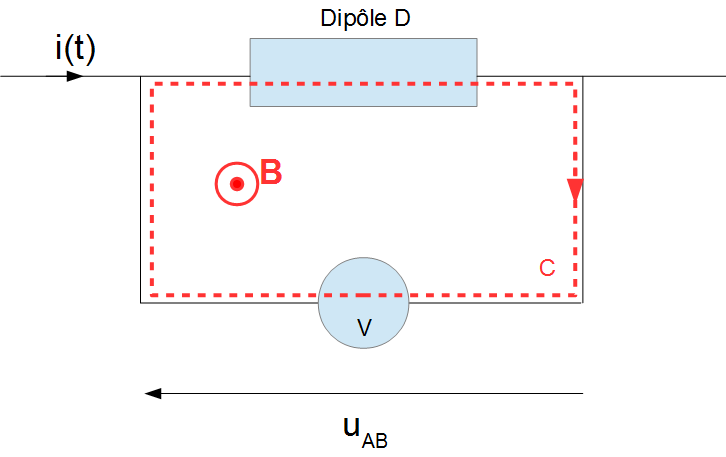
\includegraphics[scale = 0.4]{tension_variable.png}
		\caption{Mesure de la tension $u_{AB}$ en régime variable} 
		\label{fig:tension_variable}
	\end{center}
\end{figure}
Cette grandeur s'apparente à une différence de potentiel électrique en régime stationnaire, puisque $\bold{E} = \textbf{grad}\;V$. Nous allons voir que ce n'est plus le cas en régime variable, notamment en présence d'un champ magnétique. On applique la relation de Maxwell-Faraday définissant le contour $\mathcal{C}$ :
\begin{align}
	\oint_\mathcal{C}\bold{E}\cdot d\bold{r} & = \int_{\text{ADB}}\bold{E}\cdot d\bold{r} + \int_{\text{BVA}}\bold{E}\cdot d\bold{r}\\
	& = \int_{\text{ADB}}\bold{E}\cdot d\bold{r} - u_{AB}\\
	& = - \iint_\mathcal{S}\frac{\partial\bold{B}}{\partial t}\cdot d\mathcal{S}
\end{align}
D'où
\begin{equation}
	u_{AB} = \int_{\text{ADB}}\bold{E}\cdot d\bold{r} + \iint_\mathcal{S}\frac{\partial\bold{B}}{\partial t}\cdot d\mathcal{S} 
		   = \int_{\text{ADB}}\bold{E}\cdot d\bold{r} + \frac{d\Phi}{dt}
\end{equation}
la dernière égalité n'étant vraie que pour un circuit de constitution invariante dans le temps (ce qui est souvent le cas). La tension n'est plus une mesure de la différence de potentiel électrique entre $A$ et $B$ du fait de la variation temporelle du potentiel vecteur.\\

Un déplacement du voltmètre modifie en théorie la valeur de tension qu'il affiche, puisque ce déplacement altère le flux magnétique à travers la surface délimitée par le circuit. On ne peut donc mesurer une tension sans ambiguïté que si la variation temporelle de $\bold{B}$ est négligeable dans la boucle de mesure, ce qui sous entend un \textbf{régime suffisamment lentement variable}. En pratique, les champs magnétiques intenses sont localisés à l'intérieur des machines électriques et non dans la boucle de mesure, aussi ces conditions sont peu contraignantes.\\

Si le dipôle est purement résistif (résistor) de résistance $R$, on a
\begin{equation}
	u_{AB}(t) = Ri(t) + \frac{d\Phi}{dt} \simeq Ri
\end{equation}

Un dipôle purement inductif (bobine idéale) est caractérisé par
\begin{equation}
	u_{AB}(t) = \frac{d\Phi}{dt},
\end{equation}
le champ électrique à l'intérieur d'un conducteur parfait (conductivité infinie ou résistance nulle) étant nul (une bobine n'est rien d'autre qu'un fil électrique enroulé). En réalité, les bobines possèdent toujours une petite résistance interne $r$, d'où
\begin{equation}
	u_{AB}(t) = ri(t) + \frac{d\Phi}{dt},
\end{equation}

Ces expressions ne sont valables que si les grandeurs physiques sont lentement variables, ce qui est le cas pour des grandeurs électriques alternatives de fréquence 50 Hz (réseau EDF).

\subsection{Inductances}

\subsubsection{Auto-induction et inductance propre}

Tout circuit parcouru par un courant électrique d'intensité $I$ crée un champ magnétique dans lequel il est plongé. Le flux $\Phi$ de ce champ à travers le circuit (\textbf{flux propre}) est proportionnel à $I$, et on définit 
\begin{equation}
	L \equiv \frac{\Phi}{I},
\end{equation}
où $L$ est appelé coefficient d'\textbf{inductance propre} (ou d'auto-induction), mesuré en Henry (H) dans le système international. On peut démontrer que $L$ est une grandeur positive.\\

\'A titre d'exemple, calculons $L$ pour un solénoïde infini [SCH\'EMA] : le champ magnétique généré par un tel solénoïde parcouru par un courant d'intensité $I$ est uniforme à l'intérieur de la bobine et vaut
\begin{equation}
	\bold{B} = \mu_0 n I \bold{e}_z,
\end{equation}
où $n$ désigne le nombre de spires par unité de longueur ($n = N/\mathcal{L}$, $N$ étant le nombre total de spires et $\mathcal{L}$ la longueur du solénoïde) et où $\bold{e}_z$ désigne l'axe de symétrie de révolution du solénoïde, le courant étant orienté dans le sens direct par rapport à cet axe.
t
La \textbf{section du solénoïde} a prendre en compte est la \textbf{somme des sections de chaque spire traversée par le champ magnétique}\footnote{Un solénoïde n'est pas un empilement de spires contrairement à ce que l'on suppose en faisant le calcul de $\textbf{B}$, mais un seul câble décrivant une spirale.}, donc $N S$ si $S$ désigne la section du solénoïde. 
Le flux propre s'écrit donc :
\begin{equation}
	\Phi = \mu_0\frac{N^2 S}{\mathcal{L}}I,
\end{equation}
d'où le coefficient d'\textbf{inductance propre du solénoïde infini}
\begin{equation}
	L =  \mu_0\frac{N^2 S}{\mathcal{L}}.\\
\end{equation}

Donnons maintenant l'expression de la \textbf{tension aux bornes d'une bobine} en régime lentement variable :
\begin{equation}
	u_{AB}(t) = ri(t) + L\frac{di}{dt},
\end{equation}
puisque $\Phi = LI$.
Une variation du courant dans le circuit implique une variation du champ magnétique qu'il génère et donc une variation de son flux magnétique propre. D'après la loi de Faraday, une telle variation entraîne l'apparition d'une f.e.m dans le circuit. Si le courant $i(t)$ augmente, alors le flux propre $\Phi = L i(t)$ augmente aussi et la f.e.m vaut
\begin{equation}
	e(t) = - L\frac{di}{dt}
\end{equation}
si le circuit est rigide. La f.e.m est dans ce cas négative et tend à faire circuler un courant dans le sens opposé à $i$, comme prévu par la loi de Lenz. La principale conclusion de tout ceci est que \textbf{dans un circuit inductif le courant ne peut pas varier brutalement}, ce que l'on peut illustrer aisément au moyen d'une expérience. \textcolor{red}{MANIP : circuit RL parallèle avec lampe dans chaque branche. Manip qualitative.}\\

Lorsqu'on ouvre un circuit parcouru par un courant intense, le phénomène d'auto-induction s'oppose à l'extinction brutale du courant $i(t)$ (observé par exemple en débranchant un appareil en retirant la prise du mur alors qu'il est encore alimenté) et provoque parfois l'apparition d'une étincelle de rupture [PHOTO]. S'il est nécessaire d'interrompre un fort courant dans un temps très bref, il est indispensable de prendre en compte le phénomène d'auto-induction.

\subsubsection{Couplage magnétique de circuits électriques et inductance mutuelle}

Deux circuits $C_1$ et $C_2$ sont parcourus par des courants stationnaires $I_1$ et $I_2$. Chaque circuit va donc générer un champ magnétique dans lequel va baigner l'autre circuit. On définit le \textbf{coefficient d'inductance mutuelle} $M$ comme
\begin{equation}
	M \equiv \frac{\Phi_{2\rightarrow 1}}{I_2} = \frac{\Phi_{1\rightarrow 2}}{I_1}
\end{equation}
où $\Phi_{2\rightarrow 1}$ (resp. $\Phi_{1\rightarrow 2}$) désigne le flux à travers $C_1$ (resp. $C_2$) du champ magnétique $\bold{B}_2$ (resp. $\bold{B}_1$) créé par $C_2$ (resp. $C_1$). La grandeur $M$ se mesure elle aussi en Henry (H) et est une grandeur algébrique dont le signe dépend de l'orientation relative choisie pour les circuits.\\

\textbf{Exemple :} inductance mutuelle entre deux solénoïdes imbriqués [SCHEMA]

Soient deux solénoïdes de longueurs respectives $\mathcal{L}_1$ et $\mathcal{L}_2$ ($\mathcal{L}_2 \geq \mathcal{L}_1$) et de sections respectives $S_1$ et $S_2$ ($S_2 \leq S_1$) parcourus respectivement par des courants d'intensités $I_1$ et $I_2$. Le solénoïde 2 pénètre sur une longueur $h$ dans le solénoïde 1. On souhaite déterminer le coefficient d'inductance mutuelle $M$ de ce système. On utilisera le modèle du solénoïde infini pour déterminer le champ magnétique généré par chacun de ces solénoïdes.

\begin{equation}
	\Phi_{2\rightarrow 1} = \iint_{\mathcal{S}_1}\bold{B}_2\cdot d\bold{\mathcal{S}}_1
\end{equation}
où $\mathcal{S}_1$ désigne la surface du circuit constituant le solénoïde 1 traversée par le champ $\bold{B}_2$. Puisque le champ généré par un solénoïde infini est nul à l'extérieur de celui-ci, seules les spires de 1 directement en vis à vis de celles de 2 sont traversées par le flux de $\bold{B}_2$ mais seulement sur une section égale à $S_2 \times hN_1/\mathcal{L}_1$, où $\times hN_1/\mathcal{L}_1$ est le nombre de spires de 1 en vis à vis de celles de 2 sur la longueur d'interpénétration $h$. Le champ magnétique généré par 2 vaut $B_2 = \mu_0 N_2 I_2/\mathcal{2}$, d'où
\begin{equation}
	\Phi_{2\rightarrow 1} = \mu_0 \frac{hS_2 N_1 N_2}{\mathcal{L}_1\mathcal{L}_2}I_2
\end{equation}
et donc
\begin{equation}
	M = \mu_0 \frac{hS_2 N_1 N_2}{\mathcal{L}_1\mathcal{L}_2}.
\end{equation}
Un calcul similaire pour $\Phi_{1\rightarrow 2} = M/I_1$ restitue la même expression pour $M$, comme attendu. On constate que plus la longueur d'interpénétration est grande, plus $M$ l'est aussi.\\

On définit
\begin{equation}
	k \equiv \frac{M}{\sqrt{L_1L_2}}
\end{equation}
le \textbf{facteur de couplage magnétique} entre les deux circuits. Il est possible de démontrer que $k \leq 1$. Dans l'exemple évoqué plus haut, on montre que
\begin{equation}
	k = \frac{h}{\sqrt{\mathcal{L}_1\mathcal{L}_2}}\sqrt{\frac{S_2}{S_1}} \leq 1,
\end{equation}
puisque $h \leq \mathcal{L}_1 \leq \mathcal{L}_2$ et $S_2 \leq S_1$. Si $\mathcal{L}_1 = \mathcal{L}_2$ et $S_2 = S_1$, $k = 1$ et on parle de \textbf{couplage serré} (le couplage est lâche si $k \ll 1$. Dans le cas du couplage serré, la totalité du flux de $\bold{B_2}$ traverse le solénoïde 1 et vice versa (on rappelle qu'on suppose des solénoïdes infinis, qui gardent dans le volume qu'ils délimitent l'énergie magnétique qu'ils créent). Il n'y a donc pas de pertes d'énergie magnétique vers l'extérieur, car celle-ci ne fait que passer d'un solénoïde à l'autre au gré des variations d'intensité.

\newpage
\subsubsection{Le transformateur électrique}

Le couplage magnétique par induction de circuits électriques a de très nombreuses applications dans la vie quotidienne. L'une des plus importantes est le transformateur électrique. Un transformateur électrique permet de modifier les valeurs de tension et d'intensité du courant délivrées par une source d'énergie électrique alternative, en un système de tension et de courant de valeurs différentes, mais de même fréquence et de même forme. Ceci est très important dans la distribution du courant électrique : le transport sur de longues distances étant moins coûteux lorsque la tension utilisée est plus grande, des transformateurs élèvent jusqu'à 400 kV la tension alternative de 25 kV délivrée en sortie de centrale nucléaire. Pour une utilisation domestique, il faut réaliser l'opération inverse et ramener la tension à 220 V. On utilise plusieurs échelons de transformation pour cela.\\

Dans un transformateur statique, l'énergie est transférée d'un enroulement (une bobine de $N_1$ spires, souvent en cuivre) dit \textbf{primaire} à l'enroulement dit \textbf{secondaire} (une autre bobine en cuivre, mais de $N_2$ spires) par l'intermédiaire du \textbf{circuit magnétique} que constitue la carcasse du transformateur. Les deux \textbf{enroulements sont couplés par induction mutuelle} et ne sont pas reliés électriquement. Le rendement de l'installation et d'autant plus bon que le couplage entre les circuits est serré ($k \simeq 1$). Pour améliorer ce rendement, le circuit magnétique est conçu en matériau ferromagnétique (généralement du fer doux) ce qui permet de canaliser le champ magnétique généré par les enroulements à l'intérieur du circuit magnétique).

\begin{figure}[h!]
	\begin{center}
		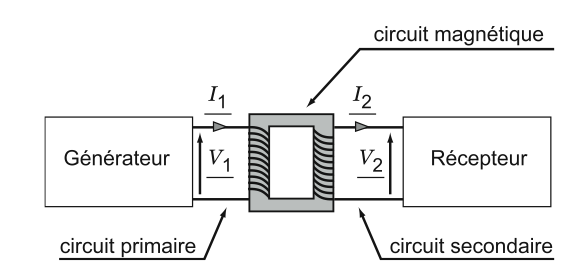
\includegraphics[scale = 0.4]{transfo.png}
		\caption{Représentation simplifiée d'un transformateur électrique} 
		\label{fig:transfo}
	\end{center}
\end{figure}

On suppose que la résistance interne des enroulements est négligeable et on néglige tout phénomène d'induction dans le circuit magnétique. Ainsi
\begin{equation}
	u_1 \simeq \frac{d\Phi_1}{dt} = L_1 \frac{d i_1}{dt} + M\frac{d i_2}{dt}  \qquad \text{et} \qquad 
	u_2 \simeq \frac{d\Phi_2}{dt} = L_2 \frac{d i_2}{dt} + M\frac{d i_1}{dt}.
\end{equation}

On trouve alors 
\begin{equation}
	u_2 = \frac{M}{L_1}u_1 + \left(\frac{L_1 L_2 - M^2}{L_1}\right)\frac{di_2}{dt}.
\end{equation}
En supposant un couplage serré, $|M| \simeq \sqrt{L_1 L_2}$ et donc
\begin{equation}
	\frac{u_2(t)}{u_1(t)} \simeq \frac{M}{L_1}.
\end{equation}
Ceci est le rapport de transformation du transformateur supposé idéal.\\

On suppose maintenant que le transformateur fonctionne à vide ($i_2 = 0$). Puisque $k = 1$, le flux $\Phi$ à travers la section des deux solénoïdes est le même et est proportionnel à $i_1$. Ainsi le flux total à travers le premier vaut $N_1\Phi$ et celui à travers le second vaut $N_2\Phi$ d'où
\begin{equation}
	L_1 = \frac{N_1 \Phi}{i_1} \qquad \text{et} \qquad M = \frac{N_2 \Phi}{i_1},
\end{equation}
d'où l'expression du rapport de transformation du transformateur idéal
\begin{equation}
	\frac{u_2(t)}{u_1(t)} \simeq \frac{N_2}{N_1}.\\
\end{equation}

\newpage
En réalité, il existe plusieurs sources de pertes dans un transformateur. Voici les principales :
\begin{itemize}
	\item \textbf{les pertes fer :} ce sont les pertes dans le circuit magnétique. Leur origine physique est double : les courants induits (on parle souvent de courants de Foucault) générés dans le noyau de fer doux (celui-ci étant résistif, il s'échauffe par effet Joule) et les pertes par hystérésis causées par le changement de direction permanent du flux magnétique dans un matériau ferromagnétique \textcolor{red}{(ce point sera abordé ultérieurement dans une autre leçon)}. On minimise ces pertes en choisissant un matériau ferromagnétique doux (réduction des pertes par hystérésis) et en privilégiant un circuit magnétique constitué de tôles isolées électriquement les unes des autres (feuilletage, pour réduire les pertes par courants de Foucault).
	\item \textbf{les pertes cuivre :} ce sont les pertes par effet Joule dans les enroulements, qui possèdent eux aussi une résistance interne.
	\item \textbf{les fuites de flux :} on considère dans notre modèle que le flux est entièrement canalisé par le circuit magnétique, ce qui n'est pas le cas. 
	Le flux circule donc partiellement hors du noyau.
\end{itemize}

\section{Conclusion}

De nombreuses applications techniques (certaines seront étudiées plus en détail en travaux dirigés) utilisent le phénomène d'induction électromagnétique. On citera notamment :
\begin{itemize}
	\item le four et les plaques à induction (couplage entre une bobine et le métal liquide/la casserole qui forment le circuit secondaire),
	\item le freinage par induction,
	\item la pince ampèremétrique [PHOTO], pour mesurer l'intensité d'un courant variable circulant dans un fil sans avoir à connecter un ampèremètre,
\end{itemize}

On retiendra trois points importants :
\begin{itemize}
	\item la variation du flux magnétique à travers un circuit conducteur entraîne l'apparition d'une force électromotrice induite dans le conducteur, susceptible de mettre en mouvement 
	les électrons : c'est le phénomène d'induction. Le flux magnétique peut varier si le champ magnétique est variable, si le circuit se déplace ou se déforme;
	\item sur un plan qualitatif, la loi de Lenz (et sur un plan quantitatif la loi de Faraday) permet de prévoir le phénomène d'induction pourvu que la forme du circuit soit invariante 
	dans le temps; 
	\item la relation de Maxwell-Faraday, qui est l'une des quatre équations de Maxwell et dont l'utilité ne se limite pas aux phénomènes d'induction;
\end{itemize}

\newpage
\section{Annexes}
\subsection{Champ magnétique généré par une bobine infinie}

		\begin{figure}[h!]
		\begin{center}
			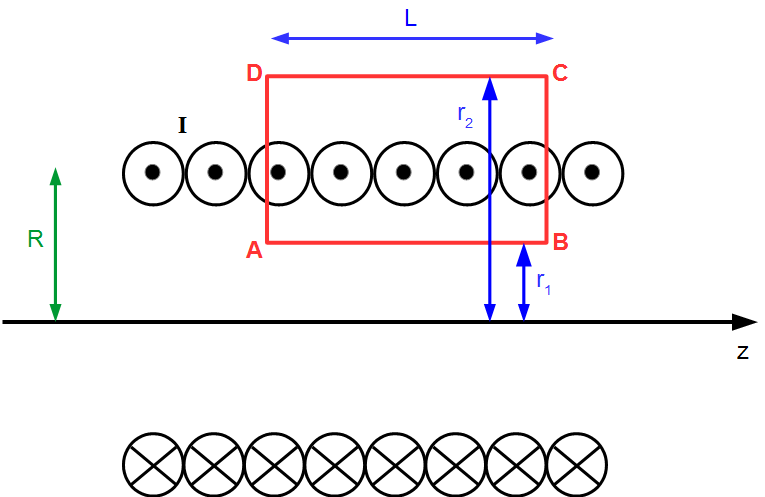
\includegraphics[scale = 0.4]{solenoid_infini.png}
			\caption{Solénoïde infini} 
			\label{fig:solenoid_infini}
		\end{center}
		\end{figure}

On se place en coordonnées cylindriques au vu de la symétrie du problème et on applique le théorème d'Ampère (équation de Maxwell-Ampère sous forme intégrale, en régime stationnaire) au contour rouge $\mathcal{C} \equiv ABCD $ :
\begin{equation}
	\oint_\mathcal{C}\bold{B}\cdot d\bold{r} = \mu_0 \iint_{\mathcal{S}/\mathcal{C}}\bold{J}\cdot d\bold{S}.
\end{equation}

Soit M un point courant du contour $\mathcal{C}$ et $\bold{B}(M)$ le champ magnétique en ce point. Tout plan passant par M et perpendiculaire à l'axe $z$ est un plan de symétrie de la distribution de courant. Ainsi, au point M, le champ magnétique est perpendiculaire à ce point :
\begin{equation}
	\bold{B}(M) = B(M) \bold{e}_z 
\end{equation}
La distribution de courant est invariante par rotation autour de l'axe $z$ et par translation le long de cet axe. La valeur de $\bold{B}$ en M ne dépend donc que de la distance de M par rapport à l'axe $z$, que l'on note $r$ :
\begin{equation}
	\bold{B}(M) = B(r) \bold{e}_z.
\end{equation}

Explicitons les deux intégrales du théorème d'Ampère. Commençons par le membre de gauche :
\begin{equation}
	\oint_\mathcal{C}\bold{B}\cdot d\bold{r} = \int_{A}^{B} B(r_1) dz + \int_{D}^{A}  B(r_2) dz = L \left( B(r_1) - B(r_2) \right).
\end{equation}
puisque $\bold{B}$ est perpendiculaire au déplacement élémentaire le long des côtés BC et DA du contour $\mathcal{C}$.
\textit{Remarque : l'élément de longueur $d\bold{r}$ en tout point de $\mathcal{C}$ est orienté selon le sens de parcours de $\mathcal{C}$.}

La valeur du membre de droite dépend de la position du contour par rapport au solénoïde. Du fait de la symétrie cylindrique du problème, on ne s'intéressera qu'au demi-plan supérieur par rapport à l'axe $z$. Trois cas sont possibles :
\begin{itemize}
	\item $r_1$ et $r_2 < R$ : le contour $\mathcal{C}$ n'entoure pas de courant électrique, par conséquent 
		\begin{equation}
			\iint_{\mathcal{S}/\mathcal{C}}\bold{J}\cdot d\bold{S} = 0
		\end{equation}
		et donc
		\begin{equation}
			B(r_1) = B(r_2).
		\end{equation}
		Le champ magnétique est uniforme dans le solénoïde puisque cette équation est valable quelque soient $r_1$ et $r_2$ inférieurs au rayon de la bobine.\\
		 
	\item $r_1 < R$ et $r_2 > R$ : le contour $\mathcal{C}$ entoure un courant électrique, donc
		\begin{equation}
			\iint_{\mathcal{S}/\mathcal{C}}\bold{J}\cdot d\bold{S} = n I L,
		\end{equation}
		où $n$ désigne le nombre de spires par unité de longueur ($nL$ est le nombre de spires entourées par le contour). On a donc
		\begin{equation}
			B(r_1) - B(r_2) = \mu_0 n I .
		\end{equation}

	\item $r_1$ et $r_2 > R$ : le contour, placé à l'extérieur du solénoïde, ne contient pas de courant électrique. On a donc à nouveau
		\begin{equation}
			B(r_1) = B(r_2),
		\end{equation}
		ce qui traduit l'uniformité du champ magnétique hors du solénoïde, y compris en un point situé infiniment loin du système. L'énergie magnétique contenue dans un volume quelconque est 		proportionnelle au carré de la norme du champ magnétique et au volume si $B$ est uniforme. Or cette grandeur doit être finie. Ceci implique $B = 0$ hors du solénoïde.
\end{itemize}

On en déduit que 
\begin{equation}
	\bold{B} = \mu_0 n I \bold{e}_z \qquad \text{dans le solénoïde}
\end{equation}
et 
\begin{equation}
	\bold{B} = 0 \qquad \text{hors du solénoïde.}
\end{equation}

Ceci n'est valable que pour un solénoïde de longueur infinie (et donc valable uniquement à l'intérieur de la bobine et loin des sections d'entrée et de sortie pour un solénoïde de longueur finie). Les lignes de champ ne quittent pas le solénoïde puisque celui-ci est infini. Pour un solénoïde réel, le champ magnétique (et son flux) est rayonné dans tout l'espace. Loin du solénoïde, il est similaire à celui d'un dipôle magnétique.  

\end{document}